\documentclass[12pt]{article}
	
\usepackage[margin=1in, left=0.6in, right=0.6in]{geometry}
\usepackage{fancyhdr}	% header
\usepackage{hyperref} % links

%\usepackage[edges]{forest}
%\usepackage{tikz-qtree}

\usepackage{amsmath,amsthm,amssymb}	%math stuff
\usepackage{graphicx} \graphicspath{ {./images/} }
%\usepackage{array}
\usepackage{setspace} % increase line spacing
\usepackage{tabularx} % long tables
\usepackage{enumitem} % labelling itmes
\usepackage{color}
% \usepackage{relsize} 
\usepackage{lmodern} % bolding \texttt{}
\usepackage[T1]{fontenc} % for {} in \texttt{}
\usepackage{listings}

\definecolor{dkgreen}{rgb}{0,0.6,0}
\definecolor{gray}{rgb}{0.5,0.5,0.5}
\definecolor{mauve}{rgb}{0.58,0,0.82}
\definecolor{backcolour}{rgb}{0.95,0.95,0.92}

% \lstset{
% 	frame=tb,
%   language=Python,
%   aboveskip=3mm,
%   belowskip=3mm,
%   showstringspaces=false,
%   columns=flexible,
%   basicstyle={\small\ttfamily},
%   numbers=none,
%   numberstyle=\tiny\color{gray},
%   keywordstyle=\color{blue},
%   commentstyle=\color{dkgreen},
%   stringstyle=\color{mauve},
%   breaklines=true,
%   breakatwhitespace=true,
%   tabsize=3
% }

\setlength{\parindent}{0pt}

\pagestyle{fancy}
\fancyhead[LO,L]{CSCB63 A1}
\fancyhead[CO,C]{Stephen Guo}
\fancyhead[RO,R]{1006313231}
\fancyfoot[LO,L]{}
\fancyfoot[CO,C]{\thepage}
\fancyfoot[RO,R]{}

\newcommand{\N}{\mathbb{N}}
\newcommand{\R}{\mathbb{R}}
\newcommand{\Rplus}{\mathbb{R}^{+}}
\newcommand{\bigbracket}[1]{\big(#1\big)}
\newcommand{\Bigbracket}[1]{\Big(#1\Big)}
\newcommand{\floorSurround}[1]{\left\lfloor#1\right\rfloor}
\newcommand{\ceilingSurround}[1]{\left\lceil#1\right\rceil}
\newcommand{\code}[1]{{\ttfamily \fontseries{b}\selectfont #1}}
% \newcommand{\code}[1]{\texttt{#1}}
\definecolor{codegray}{gray}{0.9}
% \newcommand{\code}[1]{\colorbox{codegray}{\texttt{#1}}}
\def \calO {\mathcal{O}}
\newcommand{\bigO}[1]{\ensuremath{\calO(#1)}}

\renewcommand{\qed}{\hfill$\blacksquare$}

\begin{document} %\setstretch{1.2}
%----------------------------------------------------------------------------------
%                              Table of Contents
%----------------------------------------------------------------------------------
\begin{center}
	\hypertarget{toc}{\LARGE \noindent \underline{\textbf{Table of Contents}}}\\
\end{center}

\noindent \hyperlink{2}{\textbf{Question 2:}}
\vspace{1mm}
\hrule
\vspace{1mm} \leavevmode \\

\noindent \hyperlink{3}{\textbf{Question 3:}}
\vspace{1mm}
\hrule
\vspace{1mm} \leavevmode \\

\noindent {\textbf{Question 4:}}
\vspace{1mm}
\hrule
\vspace{1mm}
\noindent\hyperlink{4.1}{(a)}\\
\hyperlink         {4.2}{(b)}\\

\noindent \hyperlink{5}{\textbf{Question 5:}}
\vspace{1mm}
\hrule
\vspace{1mm} \leavevmode \\
\newpage
%{\setstretch{1.5}$\begin{array}{r@{}>{\displaystyle}l}  \end{array}$}
%----------------------------------------------------------------------------------
%                                   Questions
%----------------------------------------------------------------------------------
%----------------------------------------------------------------------------------
% !                                    1
%----------------------------------------------------------------------------------
% \noindent \hyperlink{toc}{\hypertarget{1}{\LARGE \underline{\textbf{Question 1.}}}}
% \\\\
% \verb|ayayay 1 + 2 -> 029384|\\
% \texttt{ayayay 1 + 2 -> 029384}\\
% \code{asoidjf}\\\\
% {\ttfamily
% for (int i = 0; i < 5; i++) \{\\
% \hspace*{0mm}\ \ \ \ while (False) \{\\
% \hspace*{0mm}\ \ \ \ \ \ \ \   x += 1;\\
% \hspace*{0mm}\ \ \ \   \}\\
% \}\\\\
% }
% {\ttfamily \fontseries{l}\selectfont light}\\
% {\ttfamily \fontseries{b}\selectfont bold}\\
% {\ttfamily \fontseries{m}\selectfont medium}\\\\
% $\subset \cup\ |^{\supset}$\\
% {\ttfamily
% for (int i = 0; i < 5; i++) \{\\
% \hspace*{0mm}\ \ \ \ while (False) \{\\
% \hspace*{0mm}\ \ \ \ \ \ \ \   x += 1;\\
% \hspace*{0mm}\ \ \ \   \}\\
% \}\\\\
% }
% \code{for (int i = 0; i < 5; i++) \{\\
% \hspace*{0mm}\ \ \ \ while (False) \{\\
% \hspace*{0mm}\ \ \ \ \ \ \ \   x += 1;\\
% \hspace*{0mm}\ \ \ \   \}\\
% \}\\\\}
% $$[\kern-0.15em{\bigcap}\kern-0.8em\raisebox{0.3ex}{$\subset$}$$
% \noindent Let $n$ be arbitrary.\\

% \newpage
%----------------------------------------------------------------------------------
% !                                    2
%----------------------------------------------------------------------------------
\setstretch{1.2}
\everymath{\displaystyle} % maybe bad???
\def \imageWidth{7cm}

\noindent \hyperlink{toc}{\hypertarget{2}{\LARGE \underline{\textbf{Question 2.}}}}
\\\\
Let $n\in \N$ be arbitrary, choose $\displaystyle c=3$,\ $k=2$.
\\\\
First, add node $s$ and $t$\\
In between $s$ and $t$, add $3n$ nodes in a block with length $n$, width 3.\\
This means we have $3n + 2$ nodes.
\begin{center}
	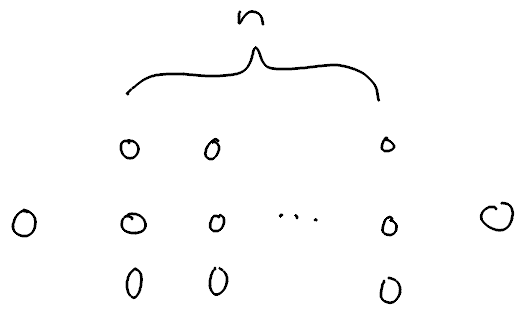
\includegraphics[width=\imageWidth]{CSCB63_A2_2-1.png}
\end{center}
For every node in a column, connect it to every node in the next column with weight $x$.
\begin{center}
	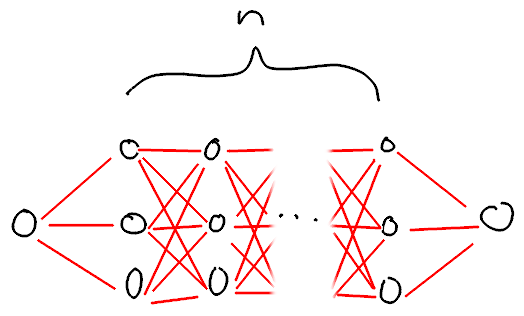
\includegraphics[width=\imageWidth]{CSCB63_A2_2-2.png}
\end{center}
Every node has 3 choices (except for the 2\textsuperscript{nd} last column of nodes). Including the first node, this will mean there is
$$\overbrace{3\times 3\times \ldots \times 3}^{n}\ =\ 3^n$$
paths from s to t, all with weight $n\times x$. This means they are all the shortest path from s to t.
\\\\
Since $n$ is arbitrary, this means that for any $n\in \N$, there is an undirected graph of $3n +2$ nodes with $3^n$ shortest path from the left-most to right-most node. \qed

\newpage
%----------------------------------------------------------------------------------
% !                                    3
%----------------------------------------------------------------------------------
\noindent \hyperlink{toc}{\hypertarget{3}{\LARGE \underline{\textbf{Question 3.}}}}
\\\\
Suppose to the contrary that given a graph $G$ with n verticies such that\\ 
for every $v \in V,\ \text{\textbf{deg($v$)}} \geq \displaystyle \frac{n}{2}$ and $G$ has > 1 connected component. 
\\\\
Then G can be split into subgraphs $S_1, \cdots,\ S_k$ such that they are all 1 connected component.
\\\\
Since all nodes have $\text{\textbf{deg($v$)}} \geq \displaystyle \frac{n}{2}$, then for all subgraphs, it must have $|S_i| \geq \displaystyle \frac{n}{2} + 1$ nodes.\\
This is because for a node to have $\text{\textbf{deg($v$)}} \geq \displaystyle \frac{n}{2}$, there must be that node, along with at least $\displaystyle \frac{n}{2}$ other nodes. 
\\\\
However, there are only $n$ nodes in the graph $G$. It is not possible for all subgraphs to have more than $\displaystyle \frac{n}{2} + 1$ if we have more than 1 subgraph. \\
This is because if we have $\geq 2$ subgraphs, then 
% set stretch broken?
{$$\begin{array}{r@{}>{\displaystyle}ll}
	|G| & {} =  |S_1| + |S_2| + \ldots + |S_k|& [\text{by given}]\\[0.5em]
	&{} \geq 2\left(\frac{n}{2} + 1\right) & [\text{at least 2 subgraphs}]\\[0.5em]
	&{} = n+2 & [\text{by algebra}]\\
\end{array}$$}
Which is a contradiction! There are only $n$ nodes in the graph $G$.
\\\\
$\therefore$ The supposition is wrong, and so $G$ must be one connect component. \qed
% $$|G| = |S_1| + |S_2| + \ldots + |S_k| \geq 2(\frac{n}{2} + 1) = n+2$$
\newpage
%----------------------------------------------------------------------------------
% !                                    4
%----------------------------------------------------------------------------------
{{\LARGE \noindent \underline{\textbf{Question 4.}}}}
\\\\
\noindent \hyperlink{toc}{\hypertarget{4.1}{(a)}}\\
In order to check if there is a cycle in a directed graph, I would use DFS with backtracking to visit all nodes. If a node has no children, it would return. Else, add the current node to the stack, then search for more children. If the current node is already in the stack, that means there is a cycle.
\begin{lstlisting}[
		% frame=tb,
		backgroundcolor=\color{backcolour},
		language=Python,
		% aboveskip=9mm,
		% belowskip=3mm,
		showstringspaces=false,
		columns=flexible,
		basicstyle={\small\ttfamily},
		% numbers=none,
		numberstyle=\tiny\color{gray},
		keywordstyle=\color{blue},
		commentstyle=\color{dkgreen},
		stringstyle=\color{mauve},
		% breaklines=true,
		numberstyle=\color{gray},
		numbersep=-17.5pt,  
		numbers=left,
		% breakatwhitespace=true,
		tabsize=5
	]
	bool hasCycle = False
	Stack stack = {}

	def traverse(Node root):
		if (root in stack): # cycle is found
			hasCycle = True
			break 

		stack.push(node)

		for node in outgoingNodes: # call traverse on all children
			traverse(node)

		stack.pop()

	traverse(root)
	return hasCycle
\end{lstlisting}
The time complexity is $\mathcal{O}(V^2+E)$. This is because there could be max $V$ elements in the stack, and it takes $\mathcal{O}{(|\text{Stack}|)}$ to search the stack. We need to search the stack after every node, so we have $\calO(V^2)$. We also have $\calO(E)$ since we we need to call \code{traverse} on every edge.
\\\\
In terms of space complexity, it would need to store the stack which could contain all nodes. So it would be $\calO(V)$

\newpage
\noindent \hyperlink{toc}{\hypertarget{4.1}{(b)}}\\
In order to get a valid ordering of the verticies, I would just use the same algorithm as \hyperlink{4.1}{(a)}. However, I would also use a queue to store the valid ordering of the verticies. For every recursive call, I would add to the queue. If a cycle is found, I would then start deleting nodes from the bottom until I get to the duplicated node. That way, It would return a valid cycle instead. 
\begin{lstlisting}[
	% frame=tb,
	backgroundcolor=\color{backcolour},
	language=Python,
	% aboveskip=9mm,
	% belowskip=3mm,
	showstringspaces=false,
	columns=flexible,
	basicstyle={\small\ttfamily},
	% numbers=none,
	numberstyle=\tiny\color{gray},
	keywordstyle=\color{blue},
	commentstyle=\color{dkgreen},
	stringstyle=\color{mauve},
	% breaklines=true,
	numberstyle=\color{gray},
	numbersep=-17.5pt,  
	numbers=left,
	% breakatwhitespace=true,
	tabsize=5
]
	Stack stack = {}
	Queue queue = {}

	def traverse(Node root):
		if (root in stack): # cycle is found
			for node in queue: # remove elements until cyclic node is found
				if node != root:
					stack.remove(node)
				else:
					queue.enqueue(node)
					return 

		stack.push(node)

		if (queue.first != queue.last): # add to queue if it's not a cycle
			queue.enqueue(node)

		for node in outgoingNodes:
			traverse(node)

		stack.pop()

	traverse(root)
	return queue
\end{lstlisting}
In terms of time complexity, it will be the same as \hyperlink{4.1}{(a)}. This is because it's the same algorithm, except we have a queue as well. \code{enqueue} takes $\calO(1)$, and removing elements will take max of \bigO{|\text{Queue}|}. Both are lower than \bigO{V^2}, so the final complexity is \bigO{V^2 + E}
\\\\
For space complexity, we will have both a queue and a stack with max $V$ elements. Therefore, the space complexity is \bigO{V}.

\newpage
%----------------------------------------------------------------------------------
% !                                    5
%----------------------------------------------------------------------------------
\noindent \hyperlink{toc}{\hypertarget{5}{\LARGE \underline{\textbf{Question 5.}}}}
\\\\
This is false.
Let $G$ be the following graph.
\begin{center}
	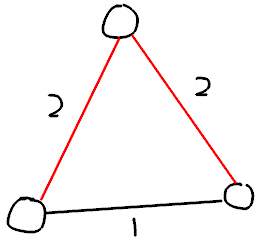
\includegraphics[width=5cm]{CSCB63_A2_5-1.png}
\end{center}\ \\
Let $T \subset E$ be the red edges.\\
$T$ is a spanning tree because it connects all of the nodes together.\\
The two red edges also belong to the two spanning trees below.
\begin{center}
	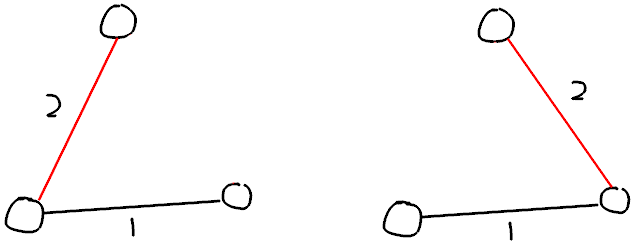
\includegraphics[width=11cm]{CSCB63_A2_5-2.png}
\end{center}\ \\
However, $T$ is not a minimum-cost spanning tree since the total weight of the edges is 4. The minimum-cost spanning tree for $G$ has weight 3.


\end{document}